Eine Signatur pr\"uft, ob ein Name an einen Wert einer angegebenen Sorte (Typ) gebunden wird. Signaturverletzungen werden protokolliert.\\
(: \auf id\zu \auf signatur\zu)\\
Bereits eingebaute Sinaturen\\
\begin{tabular}{rc|r}
natural&$\mathbb{N}$& boolean\\
integer&$\mathbb{Z}$& string\\
rational&$\mathbb{Q}$& image\\
real&$\mathbb{R}$&$\ldots$\\
numver&$\mathbb{C}$
\end{tabular}\\
(: $\ldots$) ist eine Spezialform und hat keinen Wert, aber einen Effekt: Signaturpr\"ufung\\
\underline{Prozedur Signatur} spezifizieren sowohl Signaturen f\"ur die Parameter $\text{P}_1,\text{P}_2,\ldots\text{P}_n$ als auch den Ergebniswert der Prozedur,\\
(: \auf Signatur $\text{P}_1$\zu $\ldots$ \auf Signatur $\text{P}_n$\zu $->$ \auf Signatur Ergebnis\zu)\\
Prozedur Signaturen werden \underline{bei jeder Anwendung} einer Prozedur auf Verletzung gepr\"uft. \underline{Testf\"alle} dokumentieren das erwartete Ergebnis einer Prozedur f\"ur ausgew\"ahlte Argumente:
\begin{center}
(check-expect \auf $\text{e}_1$\zu \auf
$\text{e}_2$\zu)\end{center}
Werte Ausdruck \auf $\text{e}_1$\zu \ aus und teste, ob der erhaltene Wert der Erwartung \auf $\text{e}_2$\zu \ entspricht (= der Wert von \auf $\text{e}_2$\zu) \
Einer Prozedur sollte Testf\"alle direkt vorangestellt werden.\\
Spezialform: kein Wert, sondern Effekt: Testverletzung protokollieren
\bigskip\\
\underline{Konstruktionsanleitung f\"ur Prozeduren:}
\begin{enumerate}
\item[(1)]Kurzbeschreibung (ein- bis zweizeiliger Kommentar mit Bezug auf Parametername)
\item[(2)]Signaturen
\item[(3)]Testf\"alle
\item[(4)]Prozedurrumpf
\end{enumerate}
\underline{Top-Down-Entwurf} (Programmieren durch ``Wunschdenken``)\\
Beispiel: Zeichne Ziffernblatt (Stunden- und Minutenzeiger) zu Uhrzeit h:m auf einer analogen 24h-Uhr\\
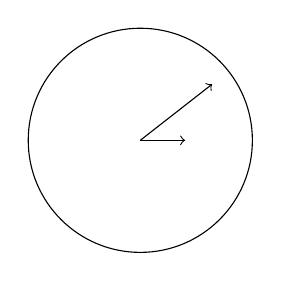
\begin{tikzpicture}
    \begin{axis}[
    legend style={draw none},
    axis equal,ymin = -2,xmin = -2,ymax = 2,
    xmax = 2,xtick ={},
    hide axis,
    xticklabels={},
    ytick ={},
    yticklabels={},
    extra x ticks={0},
    extra x tick label={},
    extra y ticks={0},
    extra y tick labels={},
    disabledatascaling,
    extra tick style = {grid = major}]
    \draw (axis cs:0,0) circle[radius=1];
    \draw[->](axis cs:0,0)--(axis cs:0.64,0.5);
    \draw[->](axis cs:0,0)--(axis cs:0.4,0);
    \end{axis}   
  \end{tikzpicture}\\
  Minutenzeiger legt $\frac{360^{\circ}}{60}$ Grad pro Minute zur\"uck (also $\frac{360}{60} \cdot m$)\\
  Studentenzeiger legt $\frac{360}{12}$ pro Stunde zur\"uck
 ($\frac{360}{12} \cdot h +\frac{360}{12} \cdot \frac{m}{60}$)
\begin{lstlisting}[frame=single]
; Grad, die Minutenzeiger pro Minute zuruecklegt
(define degrees-per-minute 360/60)

; Grad, die Stundenzeiger pro voller Stunde zuruecklegt
(define degrees-per-hour 360/12)

; Zeichne Ziffernblatt zur Stunde h und Minute m
(: draw-clock (natural natural -> image))
(check-expect (draw-clock 4 15) (draw-clock 16 15))
(define draw-clock
  (lambda (h m)
    (clock-face (position-hour-hand h m)  
    	(position-minute-hand m))))

; Winkel (in Grad), den Minutenzeiger zur Minute m einnimmt
(: position-minute-hand (natural -> rational))
(check-expect (position-minute-hand 15) 90)
(check-expect (position-minute-hand 45) 270)
(define position-minute-hand
  (lambda (m)
    (* m degrees-per-minute)))

; Winkel (in Grad), den Stundenzeiger zur Stunde h einnimmt
(: position-hour-hand (natural natural -> rational))
(check-expect (position-hour-hand 3 0) 90)
(check-expect (position-hour-hand 18 30) 195)
(define position-hour-hand
  (lambda (h m)
    (+ (* (modulo h 12) degrees-per-hour)
    ; h mod 12 in {0,1,...,11}
       (* (/ m 60) degrees-per-hour))))

; Zeichne Ziffernblatt mit Minutenzeiger um dm und
; Stundenzeiger um dh Grad gedreht
(: clock-face (rational rational -> image))
(define clock-face
  (lambda (dh dm)
    (clear-pinhole
     (overlay/pinhole
      (circle 50 "outline" "black")
      (rotate (* -1 dh) (put-pinhole 0 35 (line 0 35 "red")))
      (rotate (* -1 dm) (put-pinhole 0 45 (line 0 45 "blue")))))))
\end{lstlisting}
